% Routing games: Braess's paradox, played in the room.
% Shared preamble for the write-on class slides.
%
% Every deck is designed to be projected and annotated live on a tablet:
% whatever takes time to draw is pre-drawn, and whatever the class produces is
% left blank. Compile a deck with `pdflatex main.tex` from its own directory,
% or run `make` in decks/ to build them all.
\documentclass[10pt]{article}

\usepackage[papersize={25.6cm,14.4cm}, margin=1.1cm, bottom=1.5cm,
            footskip=0.75cm]{geometry}
\usepackage[T1]{fontenc}
\usepackage[default]{sourcesanspro}
\usepackage{newtxsf}
\usepackage{tikz}
\usepackage{amsmath}
\usepackage{parskip}
\usepackage{fancyhdr}
\usetikzlibrary{arrows.meta, positioning, calc}

\setlength{\parindent}{0pt}

% Catppuccin Latte, the palette the course site uses in its light theme, so a
% deck on the projector looks like the pages the students read.
\definecolor{inkbg}{HTML}{EFF1F5}      % base
\definecolor{inksurface}{HTML}{E6E9EF} % mantle
\definecolor{inkfaint}{HTML}{CCD0DA}   % surface2, for rules and empty boxes
\definecolor{inktext}{HTML}{4C4F69}    % text
\definecolor{inkgrey}{HTML}{8C8FA1}    % overlay1, for anything secondary
\definecolor{inkblue}{HTML}{7287FD}    % lavender, the primary accent
\definecolor{inkteal}{HTML}{179299}    % teal
\definecolor{inkred}{HTML}{FE640B}     % peach, for whatever wants attention
\definecolor{inkmauve}{HTML}{8839EF}   % mauve

\pagecolor{inkbg}
\color{inktext}

% A box to write a number into. White against the tinted page, so it reads as
% somewhere to write rather than as part of the printed material.
\newcommand{\blank}[1][1.6]{%
  \tikz[baseline=(current bounding box.base)]{%
    \draw[inkfaint, line width=0.7pt, rounded corners=2pt, fill=white]
      (0,-0.18) rectangle (#1,0.62);}}

% A ruled area to work in. Faint dots keep handwriting level on a tablet.
\newcommand{\workspace}[2]{%
  \begin{tikzpicture}
    \draw[inkfaint, line width=0.7pt, rounded corners=3pt, fill=white]
      (0,0) rectangle (#1,#2);
    \foreach \gx in {0.5,1.0,...,#1}{%
      \foreach \gy in {0.5,1.0,...,#2}{%
        \fill[inkfaint] (\gx,\gy) circle (0.5pt);}}
  \end{tikzpicture}}

% A panel for material that is printed rather than written on.
\newcommand{\panel}[2]{%
  \begin{tikzpicture}
    \draw[inkfaint, line width=0.7pt, rounded corners=3pt, fill=inksurface]
      (0,0) rectangle (#1,#2);
  \end{tikzpicture}}

% An empty payoff grid. #1 is the list of action names, #2 is drawn afterwards
% so a page can add its own marks.
\newcommand{\payoffgrid}[2]{%
  \begin{tikzpicture}[scale=1.0, every node/.style={transform shape}]
    \foreach \name [count=\j from 0] in {#1}{%
      \node[font=\bfseries, text=inkblue] at (\j*2.7+1.35,0.55) {\name};
      \node[font=\bfseries, text=inkblue] at (-1.15,-\j*2-1) {\name};
      \foreach \k [count=\i from 0] in {#1}{%
        \draw[inkfaint, line width=0.7pt, fill=white]
          (\j*2.7,-\i*2) rectangle (\j*2.7+2.7,-\i*2-2);}}
    #2
  \end{tikzpicture}}

% The five actions on a pentagon. Each action beats the one next to it and the
% one across from it, so the two winning cycles are drawn as separate panels:
% ten labelled arrows on one diagram is a tangle nobody can read from the back
% of the room.
\newcommand{\rpslscycle}[3]{%
  \begin{tikzpicture}[scale=1.0, every node/.style={transform shape},
      >={Stealth[length=2.6mm]},
      action/.style={circle, draw=inkfaint, line width=1pt, fill=white,
                     text=inktext, minimum size=1.7cm, inner sep=1pt,
                     font=\small\bfseries},
      beats/.style={->, line width=1.2pt, shorten >=3pt, shorten <=3pt,
                    draw=#1},
      word/.style={font=\scriptsize, fill=inkbg, inner sep=1.6pt, text=#1,
                   sloped, pos=#2}]
    \foreach \name/\angle in {Rock/90, Lizard/18, Spock/-54,
                              Scissors/-126, Paper/162}{%
      \node[action] (\name) at (\angle:3.1) {\name};}
    \foreach \winner/\loser/\said in {#3}{%
      \draw[beats] (\winner) -- node[word] {\said} (\loser);}
  \end{tikzpicture}}

% Running header: the deck name on the left, the page's own step on the right.
% Each deck sets its name once with \deckname.
\newcommand{\deck}{}
\newcommand{\deckname}[1]{\renewcommand{\deck}{#1}}
\newcommand{\slidehead}[1]{%
  {\small\color{inkgrey}%
   \tikz[baseline=-0.5ex]{\fill[inkblue, rounded corners=1pt]
     (0,0) rectangle (0.22,0.22);}\;\deck
   \hfill \color{inkblue}\bfseries #1}\par
  {\color{inkblue}\rule{\linewidth}{1pt}}\par\vspace{0.35em}}

\pagestyle{fancy}
\fancyhf{}
\renewcommand{\headrulewidth}{0pt}
\fancyfoot[R]{\small\color{inkgrey}\thepage}

% Deck title pages, which carry no header and no page number.
\newcommand{\titleslide}[3]{%
  \thispagestyle{empty}%
  \begin{center}
    \vspace*{\fill}
    {\Huge\bfseries\color{inkblue} #1}\\[0.7em]
    {\LARGE\color{inkgrey} #2}\\[2.4em]
    #3
    \vspace*{\fill}
  \end{center}}

% One step of the plan on a title page.
\newcommand{\stepbox}[3]{%
  \node[draw=inkblue, line width=0.9pt, rounded corners=4pt, fill=white,
        minimum width=6cm, minimum height=1.7cm, align=center,
        text=inktext] (#1) at (#2,0) {#3};}


% The base network. #1 is drawn after the fixed edges, so each page can add
% its own annotations, blanks and highlights.
\newcommand{\network}[1]{%
  \begin{tikzpicture}[
      scale=0.84, every node/.style={transform shape},
      >={Stealth[length=3mm]},
      vertex/.style={circle, draw=inkblue, line width=1.1pt, fill=white,
                     minimum size=1.05cm, font=\large\bfseries,
                     text=inkblue, inner sep=0pt},
      lab/.style={font=\small, sloped, midway},
      road/.style={->, line width=1.3pt, draw=inkgrey},
      small/.style={road, draw=inkteal, line width=1.6pt}]
    \node[vertex] (S) at (0,0) {$S$};
    \node[vertex] (A) at (4.4,2.5) {$A$};
    \node[vertex] (B) at (4.4,-2.5) {$B$};
    \node[vertex] (T) at (8.8,0) {$T$};
    \draw[small] (S) -- node[lab, below, text=inkteal] {time $=$ cars} (A);
    \draw[road] (A) -- node[lab, above] {$50$} (T);
    \draw[road] (S) -- node[lab, below] {$50$} (B);
    \draw[small] (B) -- node[lab, below, text=inkteal] {time $=$ cars} (T);
    #1
  \end{tikzpicture}}

\deckname{Routing games}

\begin{document}

% Title
\titleslide{Routing games}{Braess's paradox, in the room}{%
    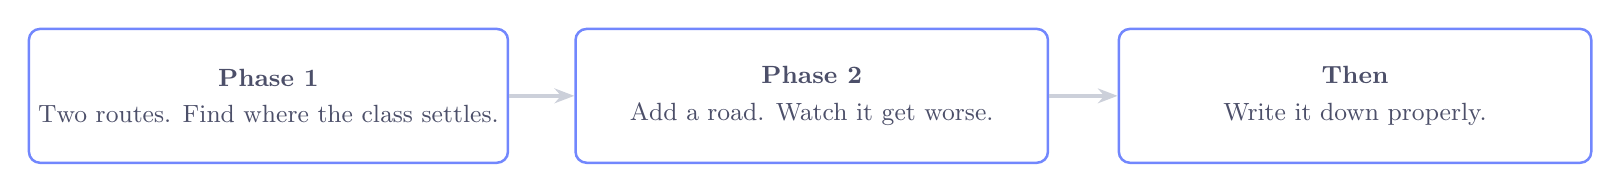
\begin{tikzpicture}[font=\small]
      \stepbox{s0}{0.0}{\textbf{Phase 1}\\[0.25em]
                          Two routes. Find where the class settles.}
      \stepbox{s1}{6.9}{\textbf{Phase 2}\\[0.25em] Add a road. Watch it get worse.}
      \stepbox{s2}{13.8}{\textbf{Then}\\[0.25em] Write it down properly.}
      \draw[-{Stealth[length=2.5mm]}, inkfaint, line width=1.2pt] (s0) -- (s1);
      \draw[-{Stealth[length=2.5mm]}, inkfaint, line width=1.2pt] (s1) -- (s2);
    \end{tikzpicture}

    \vspace{2.4em}

    {\large Drivers in the room: \blank[2.2] \hspace{2cm} Date: \blank[3]}}

\newpage
\slidehead{Phase 1: two routes}

\begin{minipage}[c]{0.60\linewidth}
\begin{center}
\network{
  \node[above left=0.1cm and 0.1cm of $(S)!0.5!(A)$]
    {\blank[1.1]\;{\color{inkgrey}\footnotesize cars}};
  \node[below right=0.1cm and 0.1cm of $(B)!0.5!(T)$]
    {\blank[1.1]\;{\color{inkgrey}\footnotesize cars}};
}
\end{center}
\end{minipage}
\hfill
\begin{minipage}[c]{0.36\linewidth}
{\large
  Top route\\[0.5em]
  \hspace*{0.6cm} \blank[1.5] $+\ 50\ =$ \blank[1.8]\\[1.6em]
  Bottom route\\[0.5em]
  \hspace*{0.6cm} \blank[1.5] $+\ 50\ =$ \blank[1.8]}
\end{minipage}

\vspace{0.15cm}

{\small\color{inkgrey} Stand on your route. Re-choose if the other one is
quicker. Stop when nobody moves.}

\vspace{0.15cm}

\hspace{0.2cm}
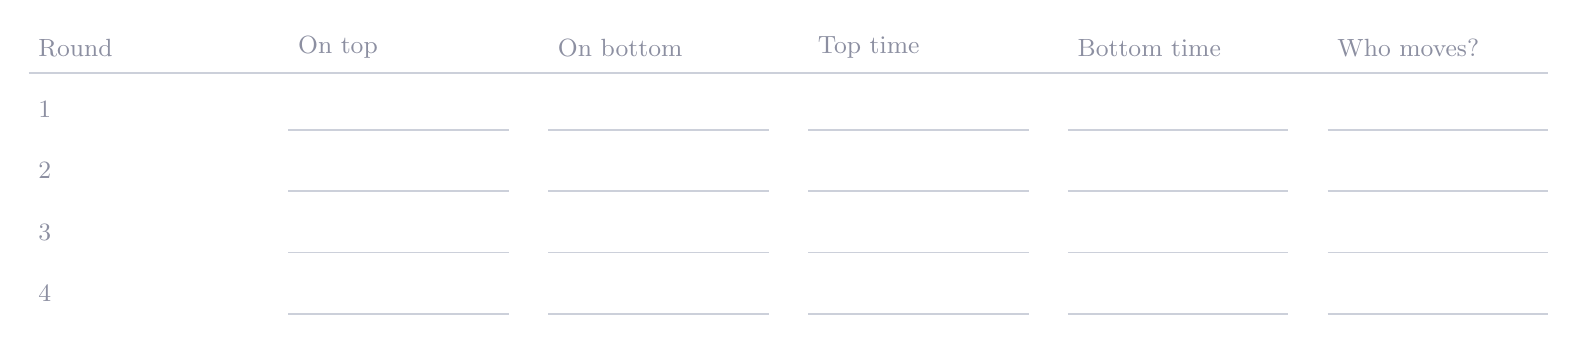
\begin{tikzpicture}[font=\small]
  \foreach \col/\lab in {0/Round, 3.3/On top, 6.6/On bottom,
                         9.9/Top time, 13.2/Bottom time, 16.5/Who moves?}{%
    \node[anchor=west, text=inkgrey] at (\col,0) {\lab};}
  \draw[inkfaint, line width=0.6pt] (0,-0.32) -- (19.3,-0.32);
  \foreach \row in {1,2,3,4}{%
    \node[anchor=west, text=inkgrey] at (0,-0.78*\row) {\row};
    \foreach \col in {3.3,6.6,9.9,13.2,16.5}{%
      \draw[inkfaint, line width=0.6pt]
        (\col,-0.78*\row-0.26) -- (\col+2.8,-0.78*\row-0.26);}}
\end{tikzpicture}

\newpage
\slidehead{Phase 1: is anybody still moving?}

\vspace{0.3cm}

{\large Where we settled: \blank[1.4] on top, \blank[1.4] on bottom.}

\vspace{0.6cm}

{\large If one driver switches from top to bottom, their time goes from
\blank[1.6] to \blank[1.6].}

\vspace{0.8cm}

{\large\bfseries So this is a \underline{\hspace{5cm}} flow.}

\vspace{0.5cm}

\begin{minipage}[t]{0.46\linewidth}
  {\small\color{inkgrey} A flow is a Nash flow when:}\\[0.4em]
  \workspace{10.6}{4.9}
\end{minipage}
\hfill
\begin{minipage}[t]{0.46\linewidth}
  {\small\color{inkgrey} Is it also the best the class could do?}\\[0.4em]
  \workspace{10.6}{4.9}
\end{minipage}

\newpage
\slidehead{Phase 2: one new road}

\vspace{0.2cm}

\begin{minipage}[c]{0.60\linewidth}
\begin{center}
\network{
  \draw[->, line width=1.6pt, draw=inkred, dashed] (A) -- (B);
  \node[right=0.15cm of $(A)!0.5!(B)$, text=inkred, font=\small]
    {new road: $0$};
  \node[above left=0.1cm and 0.1cm of $(S)!0.5!(A)$]
    {\blank[1.1]\;{\color{inkgrey}\footnotesize cars}};
  \node[below right=0.1cm and 0.1cm of $(B)!0.5!(T)$]
    {\blank[1.1]\;{\color{inkgrey}\footnotesize cars}};
}
\end{center}
\end{minipage}
\hfill
\begin{minipage}[c]{0.36\linewidth}
{\large
  $S \to A \to T$ \hspace{0.4cm} \blank[1.8]\\[1.5em]
  $S \to B \to T$ \hspace{0.4cm} \blank[1.8]\\[1.5em]
  {\color{inkred}$S \to A \to B \to T$} \hspace{0.4cm} \blank[1.8]}
\end{minipage}

\vspace{0.7cm}

{\small\color{inkgrey} Re-choose again. The new road is free, so who would not
take it?}

\vspace{0.3cm}

\begin{center}
\workspace{22.6}{2.6}
\end{center}

\newpage
\slidehead{Phase 2: where everyone ends up}

\vspace{0.8cm}

\begin{center}
{\large
  $S \to A$: \blank[1.3] cars $=$ \blank[1.3] mins
  \hspace{1.1cm} $+$ \hspace{1.1cm}
  $A \to B$: $0$ mins
  \hspace{1.1cm} $+$ \hspace{1.1cm}
  $B \to T$: \blank[1.3] cars $=$ \blank[1.3] mins}

\vspace{1.4em}

{\Large Everyone's time: \blank[2.4] mins}
\end{center}

\vspace{0.9cm}

{\large Nobody wants to leave: going back to $S \to A \to T$ would cost
\blank[1.5] $+\ 50\ =$ \blank[1.8].}

\vspace{1.1cm}

\begin{center}
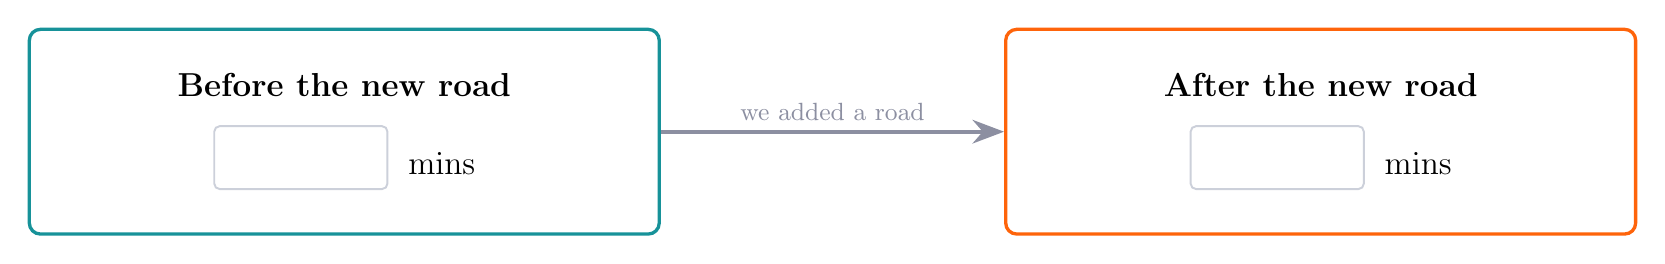
\begin{tikzpicture}[font=\large]
  \node[draw=inkteal, line width=1.2pt, rounded corners=4pt,
        minimum width=8cm, minimum height=2.6cm, align=center]
    (before) at (0,0) {\textbf{Before the new road}\\[0.8em]
                       \blank[2.2]\; mins};
  \node[draw=inkred, line width=1.2pt, rounded corners=4pt,
        minimum width=8cm, minimum height=2.6cm, align=center]
    (after) at (12.4,0) {\textbf{After the new road}\\[0.8em]
                         \blank[2.2]\; mins};
  \draw[-{Stealth[length=4mm]}, inkgrey, line width=1.4pt]
    (before) -- node[above, font=\small, text=inkgrey] {we added a road}
    (after);
\end{tikzpicture}
\end{center}

\newpage
\slidehead{Why it got worse}

\vspace{0.4cm}

{\large One more car joins a small road that already carries $x$ cars.}

\vspace{0.7cm}

\hspace{1cm}
\begin{minipage}{0.4\linewidth}
  {\large It costs \emph{me} \blank[1.6] minutes.}
\end{minipage}
\begin{minipage}{0.5\linewidth}
  {\large It costs \emph{everyone else} \blank[1.6] minutes.}
\end{minipage}

\vspace{0.9cm}

{\large I pay the first and ignore the second. The road's total time is}

\vspace{0.5cm}

\begin{center}
{\Large $x \, c(x) \;=\;$ \blank[2] \hspace{2.6cm}
 and one more car really adds
 $\dfrac{\mathrm{d}}{\mathrm{d}x}\big(x \, c(x)\big) \;=\;$ \blank[2]}
\end{center}

\vspace{0.6cm}

\begin{center}
\workspace{22.6}{2.8}
\end{center}

\newpage
\slidehead{Writing it down}

\vspace{0.3cm}

{\large A routing game has a flow $f$ on each route, and a cost}

\vspace{0.2cm}

\begin{center}
{\Large $\displaystyle C(f) \;=\; \sum_{e} f_e\, c_e(f_e)$}
\end{center}

\vspace{0.4cm}

\begin{minipage}[t]{0.47\linewidth}
  {\large Our network, \emph{before} the new road:}\\[0.5em]
  \workspace{10.8}{5}
\end{minipage}
\hfill
\begin{minipage}[t]{0.47\linewidth}
  {\large Our network, \emph{after} the new road:}\\[0.5em]
  \workspace{10.8}{5}
\end{minipage}

\newpage
\slidehead{Nash flow against optimal flow}

\vspace{0.3cm}

{\large A planner who could route us all could ignore the new road and send
half of us each way.}

\vspace{0.5cm}

\begin{minipage}[t]{0.47\linewidth}
{\large Left alone: the Nash flow \(\tilde f\), and each driver's time:}\\[0.5em]
\workspace{10.8}{4.4}
\end{minipage}
\hfill
\begin{minipage}[t]{0.47\linewidth}
{\large Planned: the optimal flow \(f^{*}\), and each driver's time:}\\[0.5em]
\workspace{10.8}{4.4}
\end{minipage}

\vspace{0.7cm}

\begin{center}
{\Large Price of anarchy \(\;=\; \dfrac{C(\tilde f)}{C(f^{*})} \;=\;
 \dfrac{\;\blank[1.8]\;}{\;\blank[1.8]\;} \;=\;\) \blank[2]}
\end{center}

\newpage
\slidehead{The same thing, as an exam answer}

\vspace{0.5cm}

{\large What we just did in the room is \textbf{Question 1} on the Routing
Games page, worth 25 marks.}

\vspace{0.9cm}

\hspace{0.6cm}
\begin{minipage}{0.92\linewidth}
{\large
\begin{tabbing}
\hspace{1.2cm} \= \hspace{17cm} \= \kill
\textbf{(a)} \> What a Nash flow is here. \> [3]\\[0.55em]
\textbf{(b)} \> The Nash flow and each driver's time. \> [5]\\[0.55em]
\textbf{(c)} \> Adding $A \to B$: show all 40 on $S \to A \to B \to T$ is a
  Nash flow. \> [7]\\[0.55em]
\textbf{(d)} \> Compare the times, and explain it through the congestion each
  driver ignores. \> [7]\\[0.55em]
\textbf{(e)} \> Compute the price of anarchy. \> [3]
\end{tabbing}}
\end{minipage}

\vspace{1.2cm}

\begin{center}
{\large\color{inkgrey} vknight.org/gt/topics/routing-games.html}
\end{center}

\end{document}
